\subsection{Experiment \rnum{2}: Anomaly Detection}

Table \ref{tab:confusion-matrix-results} presents a comparative analysis of all four models. The $\beta-CVAE$ has the highest values for the positives and the lowest of the negatives.

\begin{table}[!htbp]
\centering
\begin{tabular}{l
    S[table-format=3.0]
    S[table-format=3.0]
    S[table-format=3.0]
    S[table-format=3.0]
}
\toprule
\textbf{Model} & {\textbf{TP}} & {\textbf{FP}} & {\textbf{TN}} & {\textbf{FN}} \\
\midrule
\rowcolor{gray!10} AE   & 0 & 42 & 418 & 140 \\
$\beta$-VAE  & 101 & 2 & 458 & 39 \\
\rowcolor{gray!10} CAE  & 75 & 9 & 451 & 65 \\
$\beta$-CVAE & \textbf{103} & \textbf{5} & \textbf{455} & \textbf{37} \\
\bottomrule
\end{tabular}
\label{tab:confusion-matrix-results}
\caption{Confusion Matrix Values for all four models}
\end{table}


\begin{table}[!htbp]
\centering
\label{tab:performance-metrics}
\begin{tabular}{l
    S[table-format=1.3]
    S[table-format=1.3]
    S[table-format=1.3]
    S[table-format=1.3]
    S[table-format=1.3]
}
\toprule
\textbf{Model} & {\textbf{Precision}} & {\textbf{Recall (TPR)}} & {\textbf{F1-Score}} & {\textbf{FPR}} & {\textbf{PR AUC}} \\
\midrule
\rowcolor{gray!10} AE   & 0.000 & 0.000 & 0.000 & 0.091 & 0.157 \\
$\beta$-VAE  & \textbf{0.981} & 0.721 & \textbf{0.831} & \textbf{0.004} & \textbf{0.925} \\
\rowcolor{gray!10} CAE  & 0.893 & 0.536 & 0.670 & 0.020 & 0.736 \\
$\beta$-CVAE & 0.954 & \textbf{0.736} & \textbf{0.831} & 0.011 & 0.924 \\
\bottomrule
\end{tabular}
\label{tab:auto}
\caption{Anomaly Detection Performance Metrics Comparison}
\end{table}



\begin{figure}[!htbp]
    \centering
    \begin{subfigure}[b]{\textwidth}
        \centering
        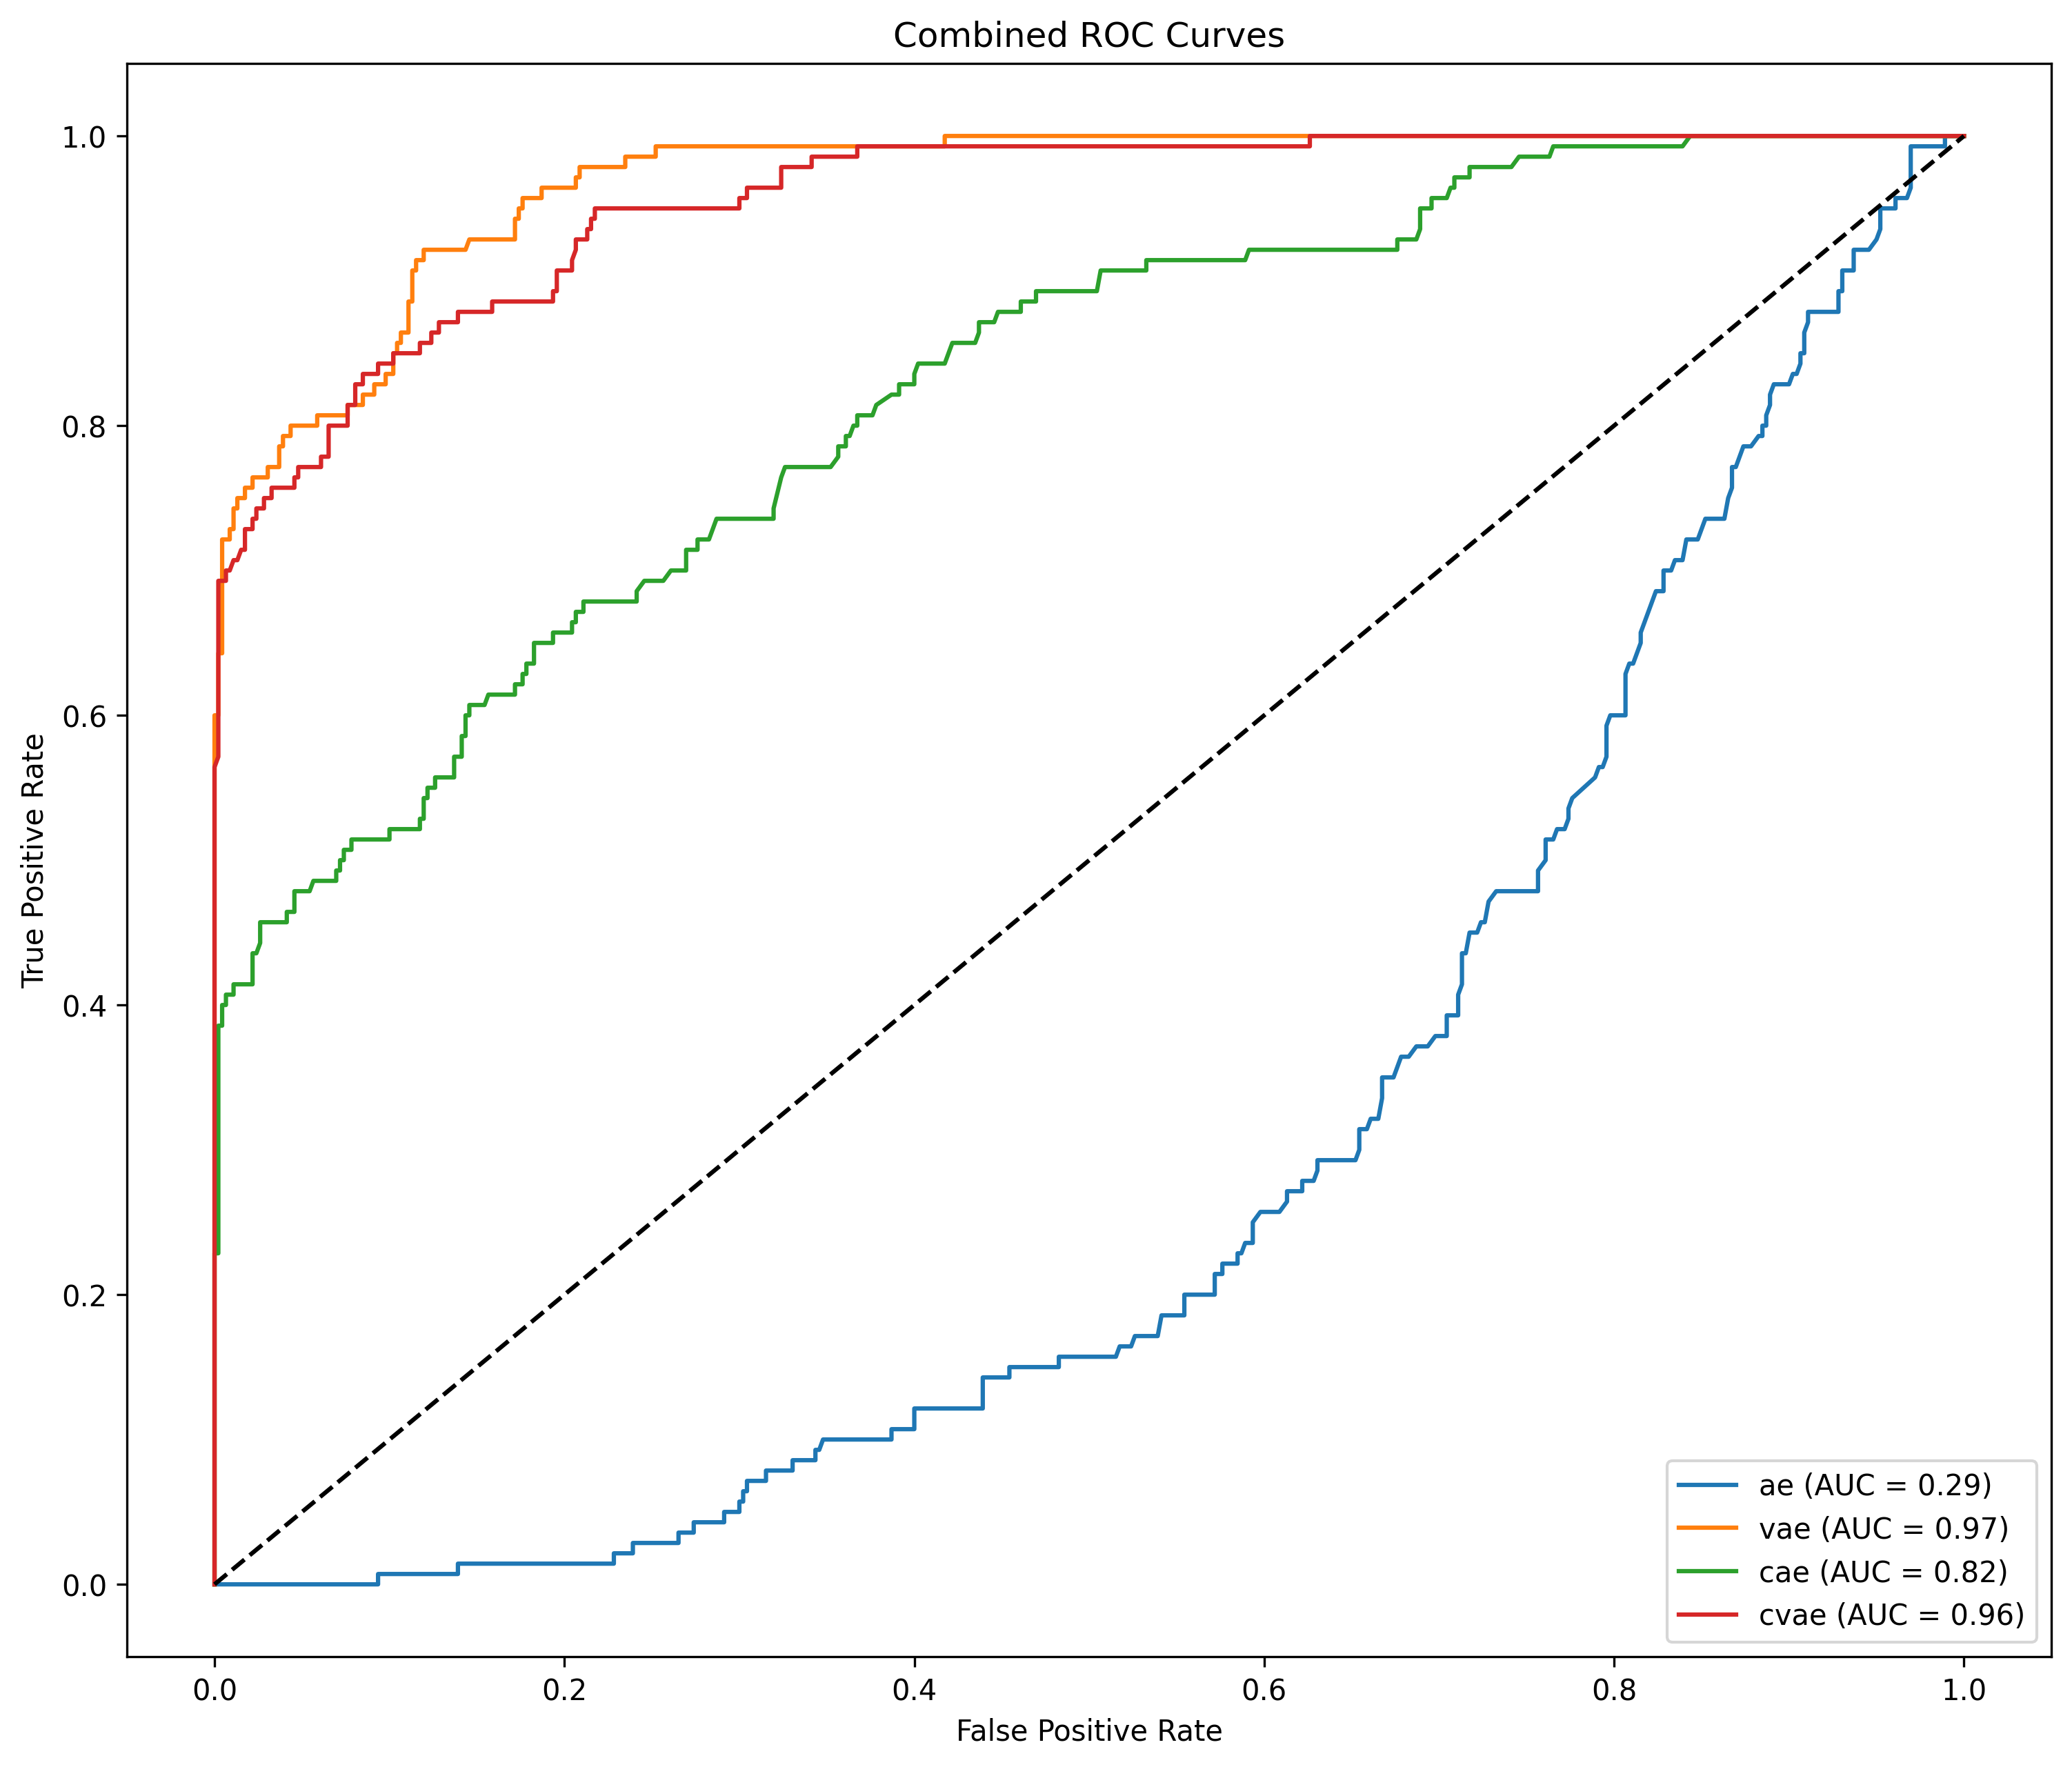
\includegraphics[width=0.8\textwidth]{figures/anomalies/combined_roc_curve.png}
        \caption{Combined ROC Curve for all models}
        \label{fig:roccurve}
    \end{subfigure}
    \vspace{1em}
    \begin{subfigure}[b]{\textwidth}
        \centering
        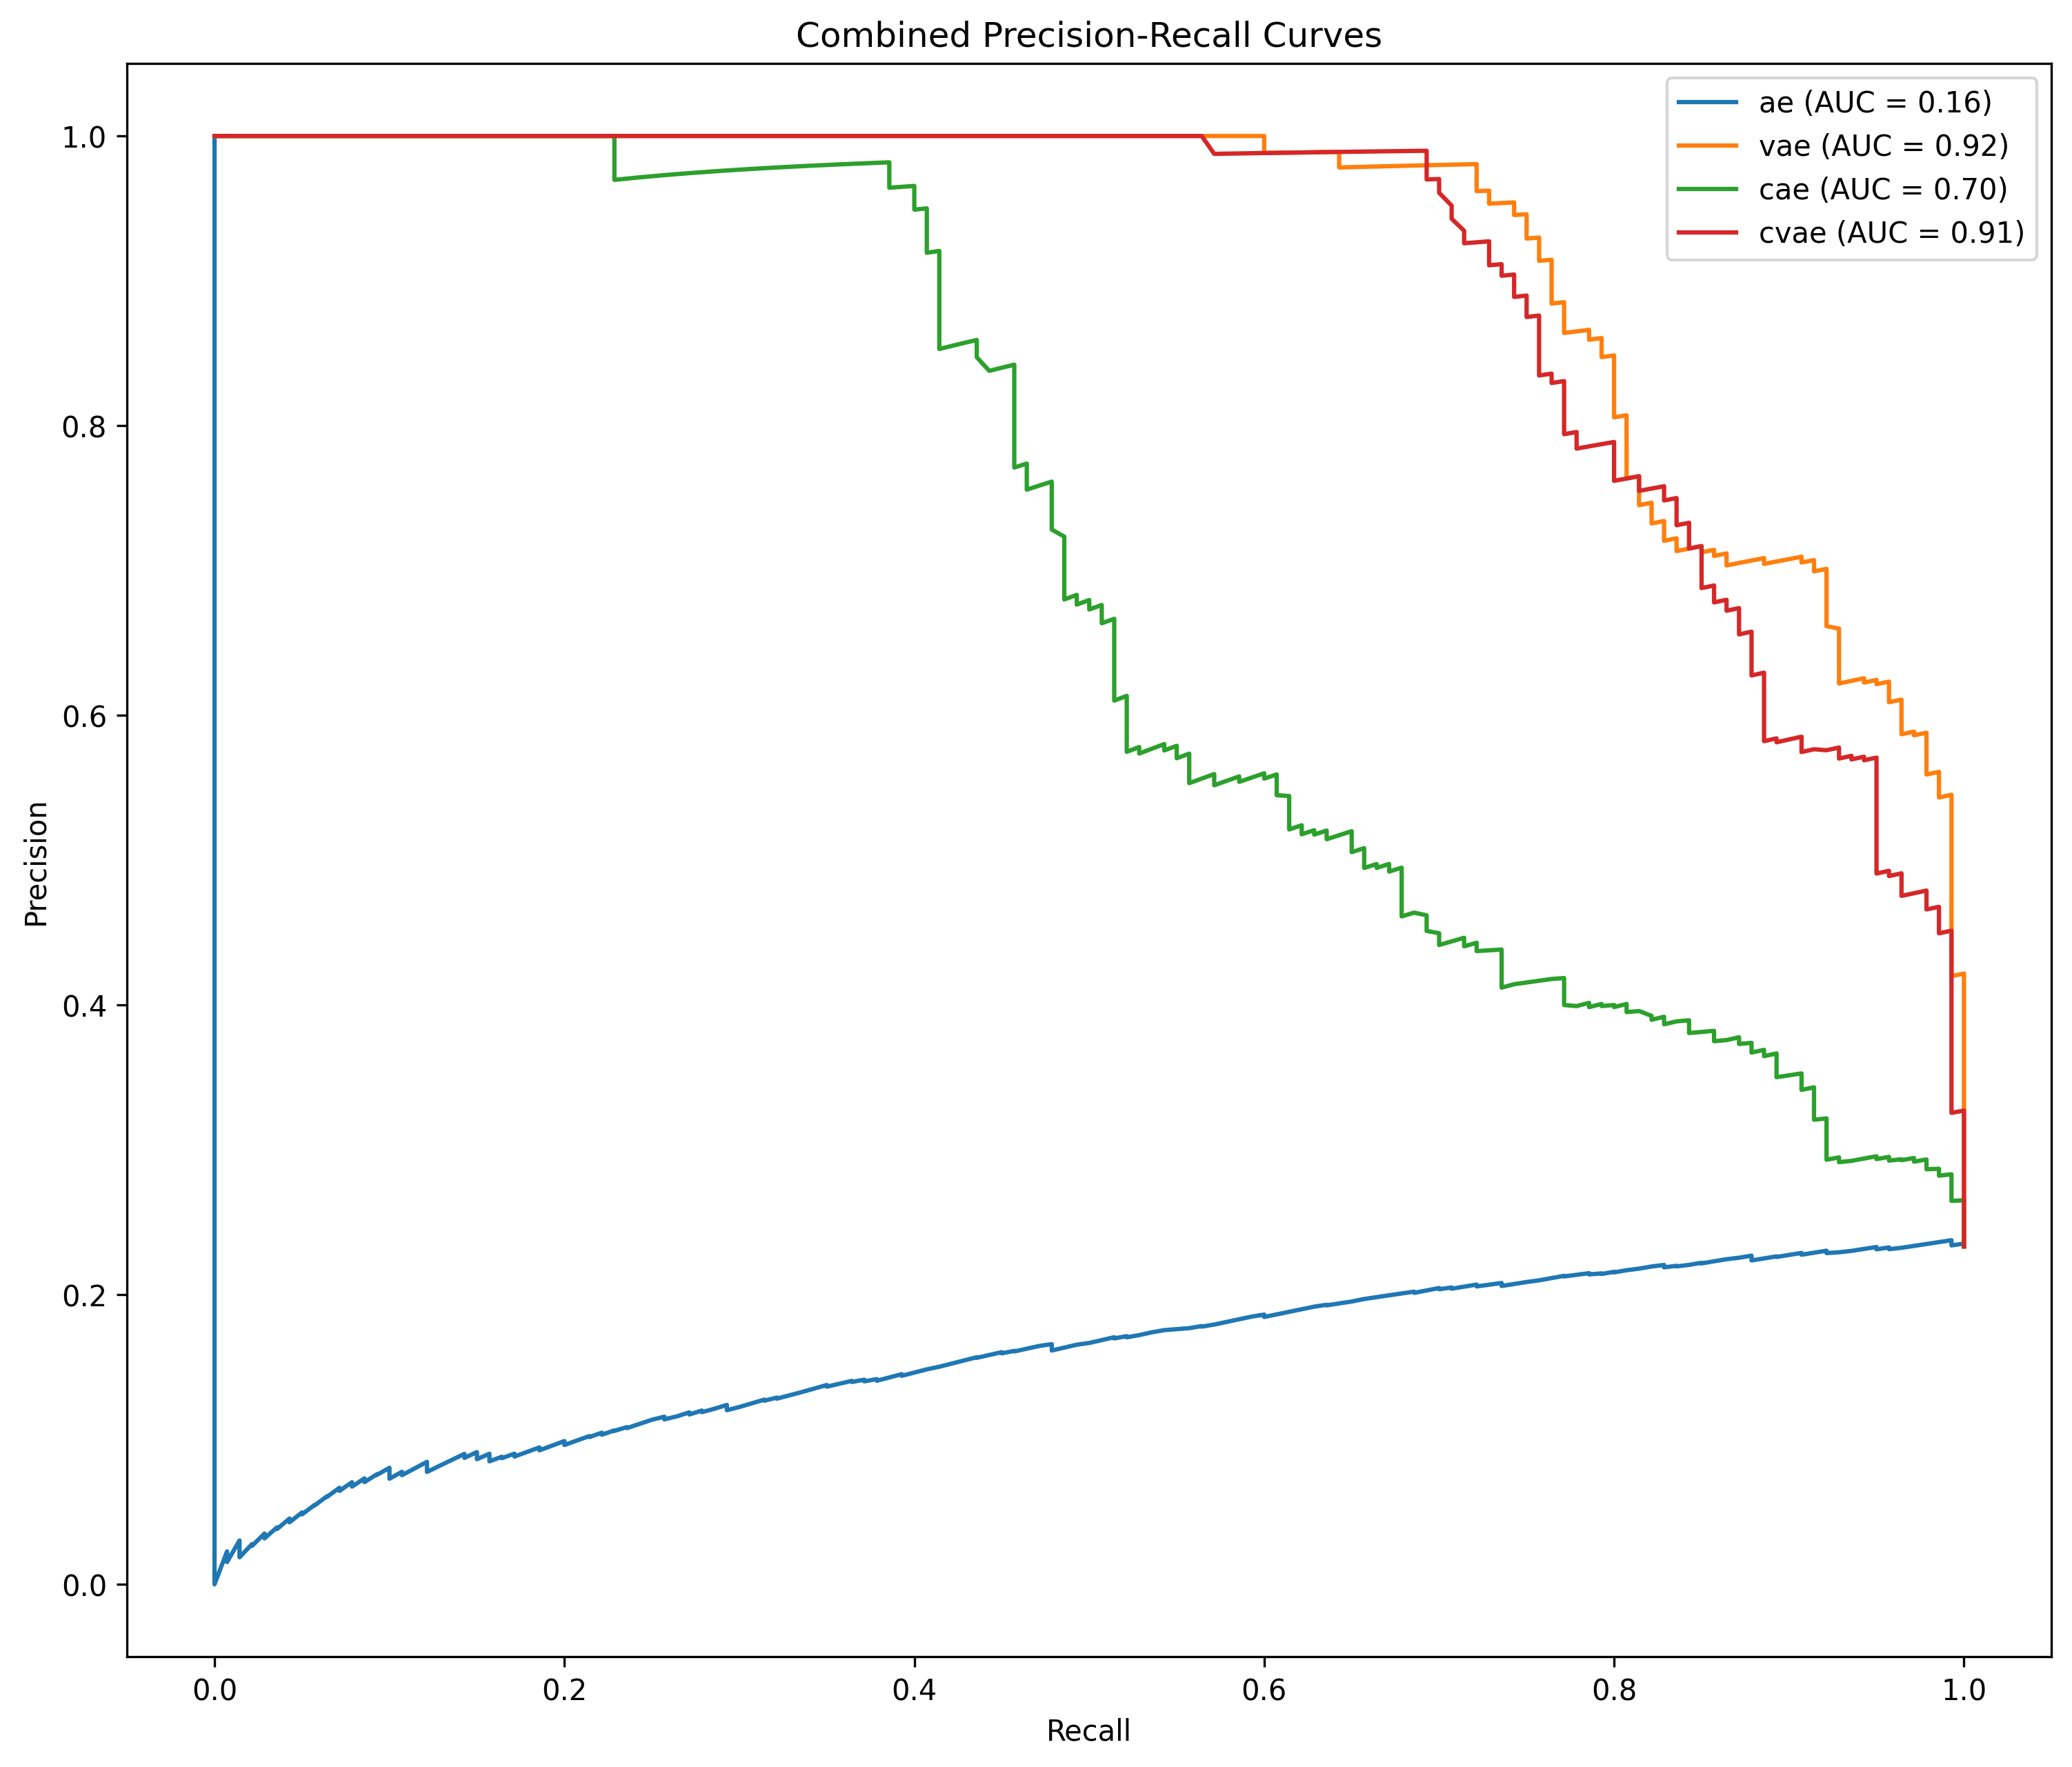
\includegraphics[width=0.8\textwidth]{figures/anomalies/combined_pr_curve.png}
        \caption{Combined PR Curve for all models}
        \label{fig:prcurve}
    \end{subfigure}
    \caption{Performance curves for all models}
    \label{fig:combined_curves}
\end{figure}
\clearpage

\subsubsection{Threshold Analysis}

\begin{figure}[!h]
  \centering
  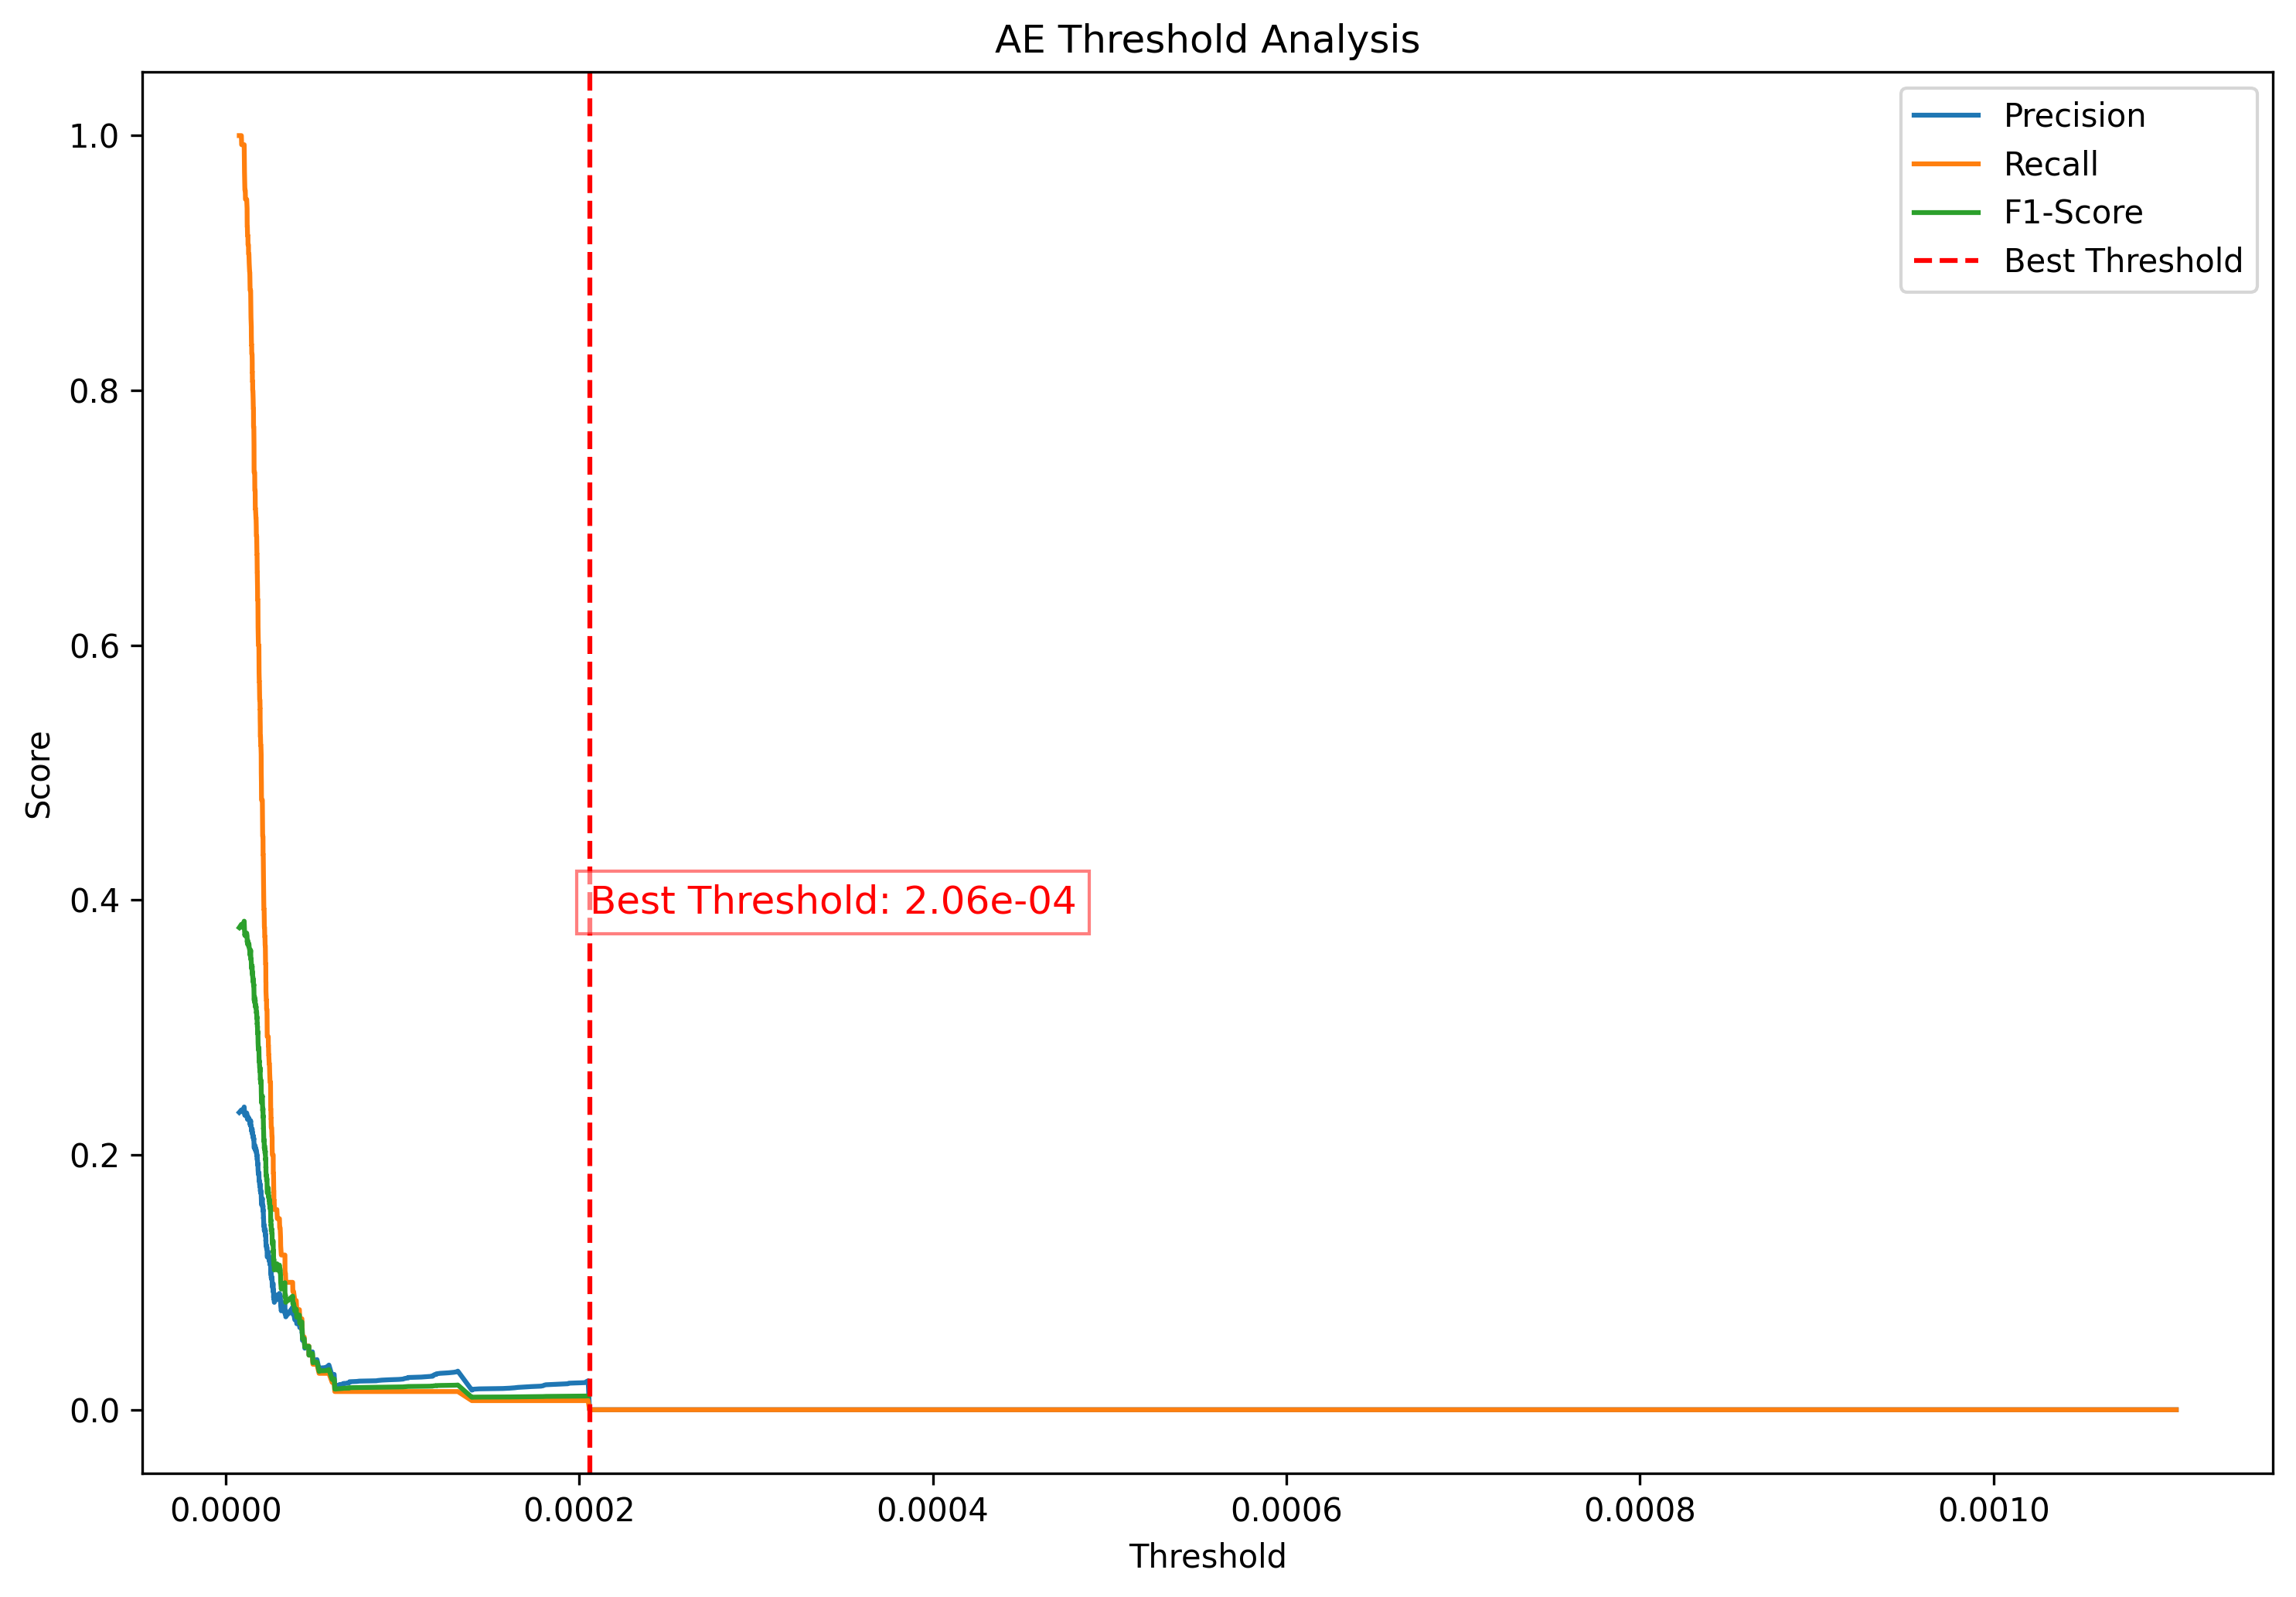
\includegraphics[scale=0.5]{figures/anomalies/ae/threshold.png}
  \caption{Threshhold analysis for the AE model}
  \label{fig:threshold_ae}
\end{figure}

\begin{figure}[!h]
  \centering
  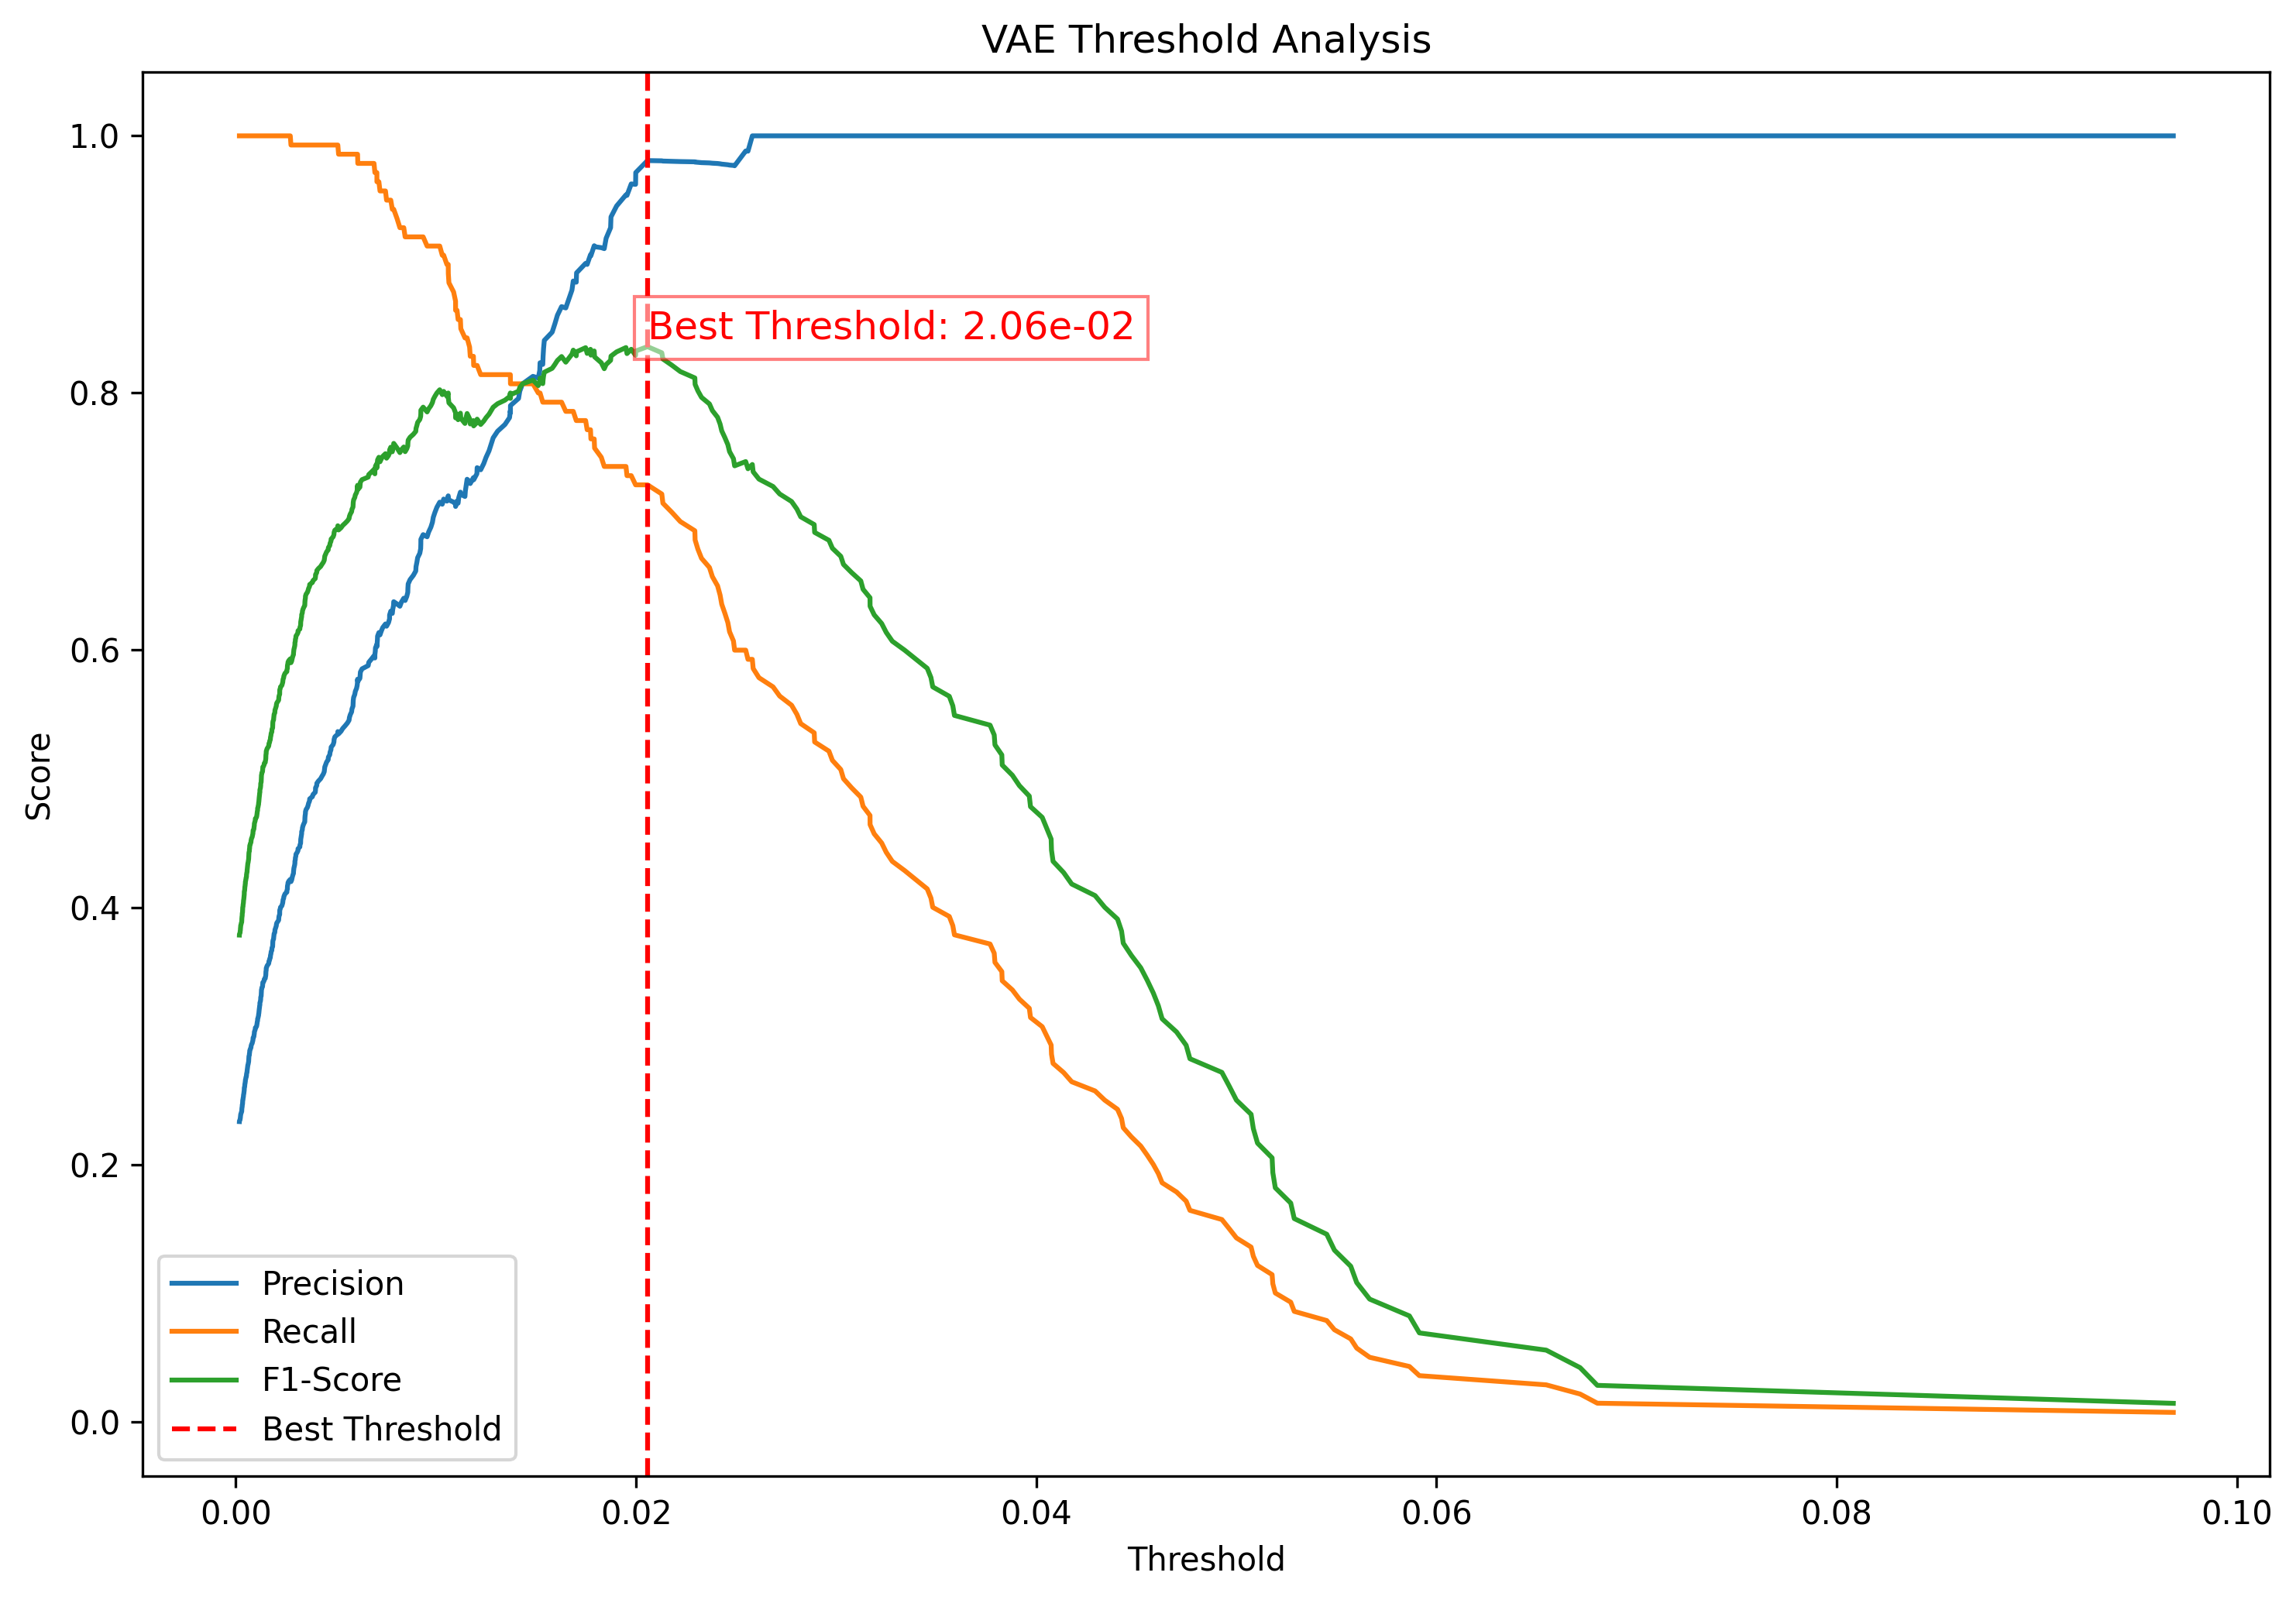
\includegraphics[scale=0.5]{figures/anomalies/vae/threshold.png}
  \caption{Threshhold analysis for the $\beta$-VAE model}
  \label{fig:threshold_vae}
\end{figure}

\begin{figure}[!h]
  \centering
  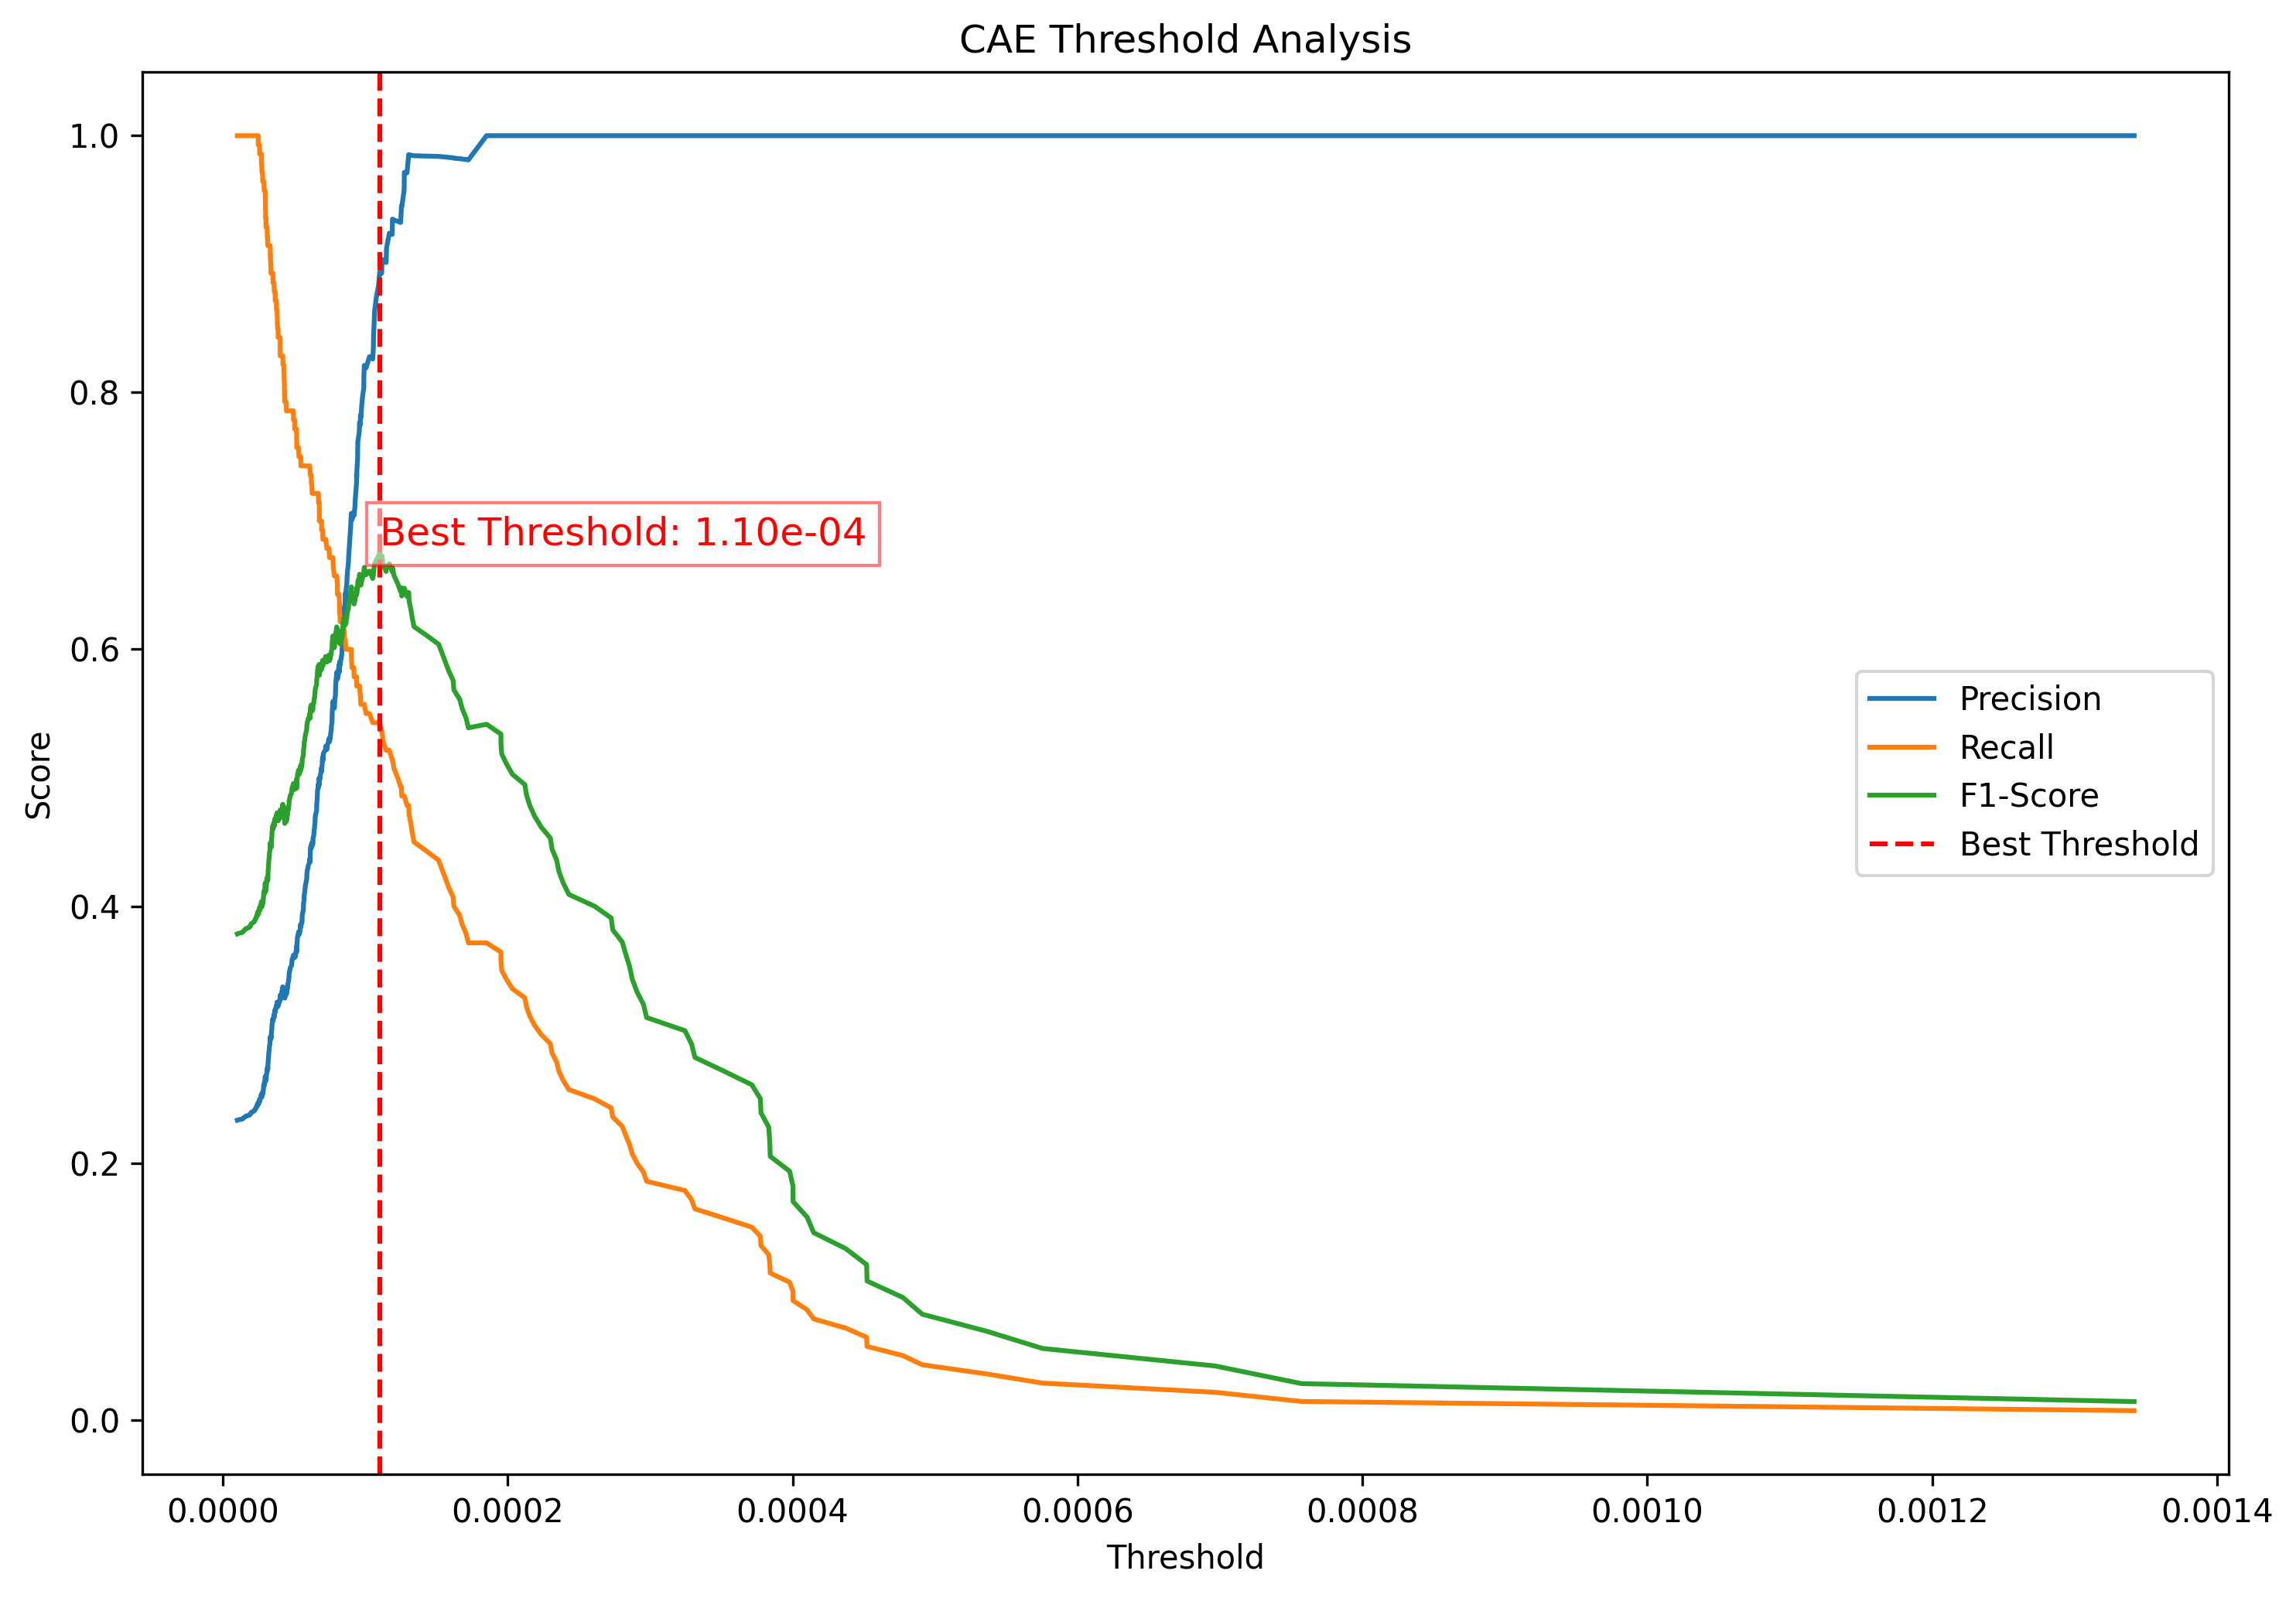
\includegraphics[scale=0.5]{figures/anomalies/cae/threshold.png}
  \caption{Threshhold analysis for the CAE model}
  \label{fig:threshold_cae}
\end{figure}

\begin{figure}[!h]
  \centering
  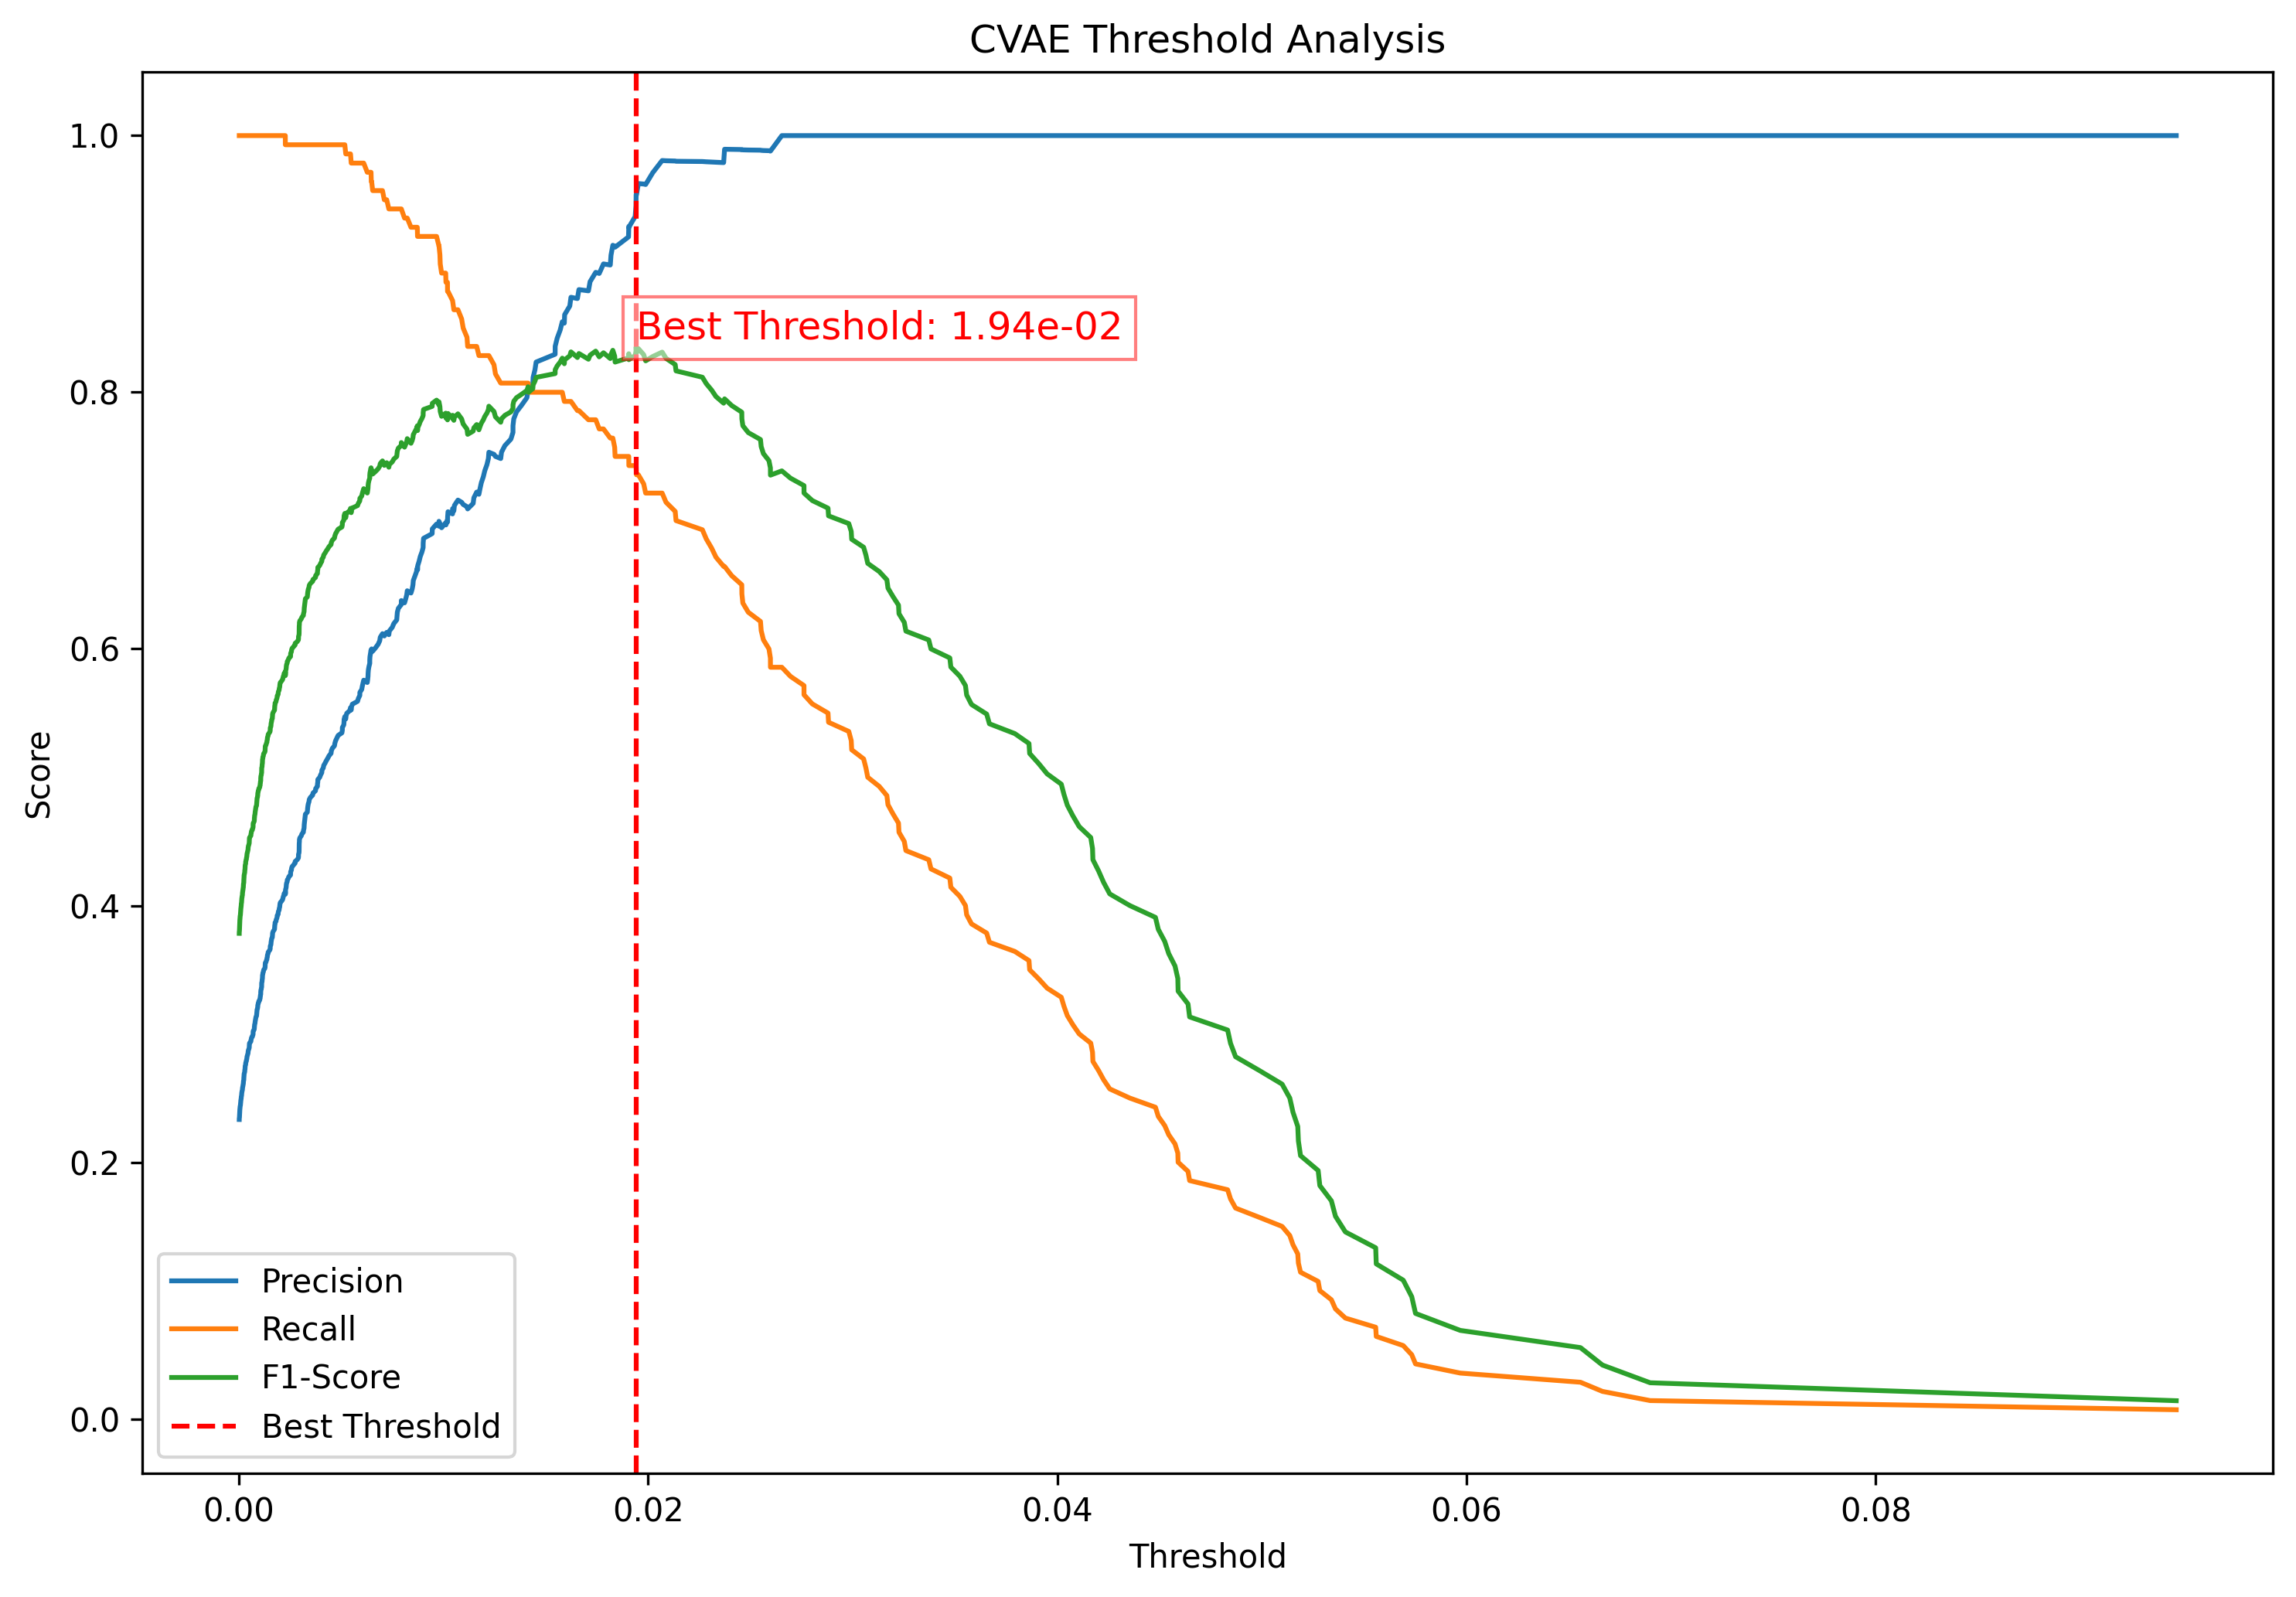
\includegraphics[scale=0.5]{figures/anomalies/cvae/threshold.png}
  \caption{Threshhold analysis for the $\beta$-CVAE model}
  \label{fig:threshold_vae}
\end{figure}